\documentclass{beamer}

% Frame Number
\setbeamertemplate{footline}[frame number]

% Input Encoding
\usepackage[utf8]{inputenc}

% PDF Bookmarks
\usepackage{url}
\usepackage{hyperref} 
\hypersetup{colorlinks}
\hypersetup{bookmarksopen}
\hypersetup{bookmarksnumbered}
\hypersetup{citecolor=blue}
\hypersetup{urlcolor=blue}
\hypersetup{linkcolor=blue}

% Spacing
\usepackage{xspace}

% Figures
\usepackage{graphicx}
\graphicspath{{../../img/}}
\usepackage{subcaption}

% Tables
\usepackage{booktabs}

% Strike Through
\usepackage{ulem}

% Code Snippet 
\usepackage{listings}
\lstset{
  belowcaptionskip=1\baselineskip,
  breaklines=true,
  frame=L,
  xleftmargin=\parindent,
  numbers=left,
  stepnumber=2,
  language=C,
  tabsize=2,
  showstringspaces=false,
  basicstyle=\footnotesize\ttfamily,
  keywordstyle=\bfseries\color{blue},
  commentstyle=\itshape\color{gray},
  identifierstyle=\bfseries\color{black},
  stringstyle=\bfseries\color{purple},
}

% Title
\title[Nanvix]{%
	\textbf{%
		The Nanvix Operating System\\
		\small{Security}
	}
}

% Authors
\author[Pedro H. Penna]{%
	Pedro H. Penna%
}

% Affiliations
\institute{
	\url{pedrohenriquepenna@gmail.com}
}

% Short-Hands
\newcommand{\ie}{\textit{ie.\xspace}}

\begin{document}

\frame{\titlepage}

\section{Barebones on Security}

	\begin{frame}
	\frametitle{Barebones on Security}
	\framesubtitle{Motivation}
	\begin{itemize}
	\setlength\itemsep{1.5em}
		\uncover<1->{
			\item Computer networks
		}

		\uncover<2->{
			\item Multiuser
		}

		\uncover<3->{
			\item Multiprogramming and time sharing
		}
	\end{itemize}
	\end{frame}

	\begin{frame}
	\frametitle{Barebones on Security}
	\framesubtitle{Rules of Thumb}
	\begin{itemize}
	\setlength\itemsep{1.5em}
			\item Data \alert<1->{confidentiality}
			\begin{itemize}
			\uncover<2->{
				\item Secrets should remain in secret
			}
			\end{itemize}

			\item Data \alert<1->{integrity}
			\begin{itemize}
			\uncover<3->{
				\item Unauthorized changes to data should be denied
			}
			\end{itemize}
			
			\item System \alert<1->{availability}
			\begin{itemize}
			\uncover<4->{
				\item Nobody can disturb the system to make it unusable
			}
			\end{itemize}
	\end{itemize}
	\end{frame}

	\begin{frame}
	\frametitle{Barebones on Security}
	\subtitle{Data Confidentiality}
	\begin{itemize}
	\setlength\itemsep{1.5em}
		\uncover<1->{
			\item Exposure of data
			\begin{itemize}
			\setlength\itemsep{0.5em}
				\item Steal passwords
				\item Retrieve classified information
			\end{itemize}
		}
		\uncover<2->{
			\item Data access grated to authorized people only
			\begin{itemize}
			\setlength\itemsep{0.5em}
				\item Owner of data may change access permissions
				\item Operating system should deny unauthorized accesses
			\end{itemize}
		}
	\end{itemize}
	\end{frame}

	\begin{frame}
	\frametitle{Barebones on Security}
	\subtitle{Data Integrity}
	\begin{itemize}
	\setlength\itemsep{1.5em}
		\uncover<1->{
			\item Tampering with data
			\begin{itemize}
			\setlength\itemsep{0.5em}
				\item Play with sensitive content
			\end{itemize}
		}
		\uncover<2->{
			\item Data may be modified only by authorized people
			\begin{itemize}
			\setlength\itemsep{0.5em}
				\item Permissions should be granted by the owner of data
				\item Substantial changes should be approved by the owner of data
				\item Operating system should deny unauthorized
				modifications
			\end{itemize}
		}
	\end{itemize}
	\end{frame}

	\begin{frame}
	\frametitle{Barebones on Security}
	\subtitle{System Availability}
	\begin{itemize}
	\setlength\itemsep{1.5em}
		\uncover<1->{
			\item Denial of service
			\begin{itemize}
			\setlength\itemsep{0.5em}
				\item Rule over some resource
				\item Make the system unavailable
			\end{itemize}
		}
		\uncover<2->{
			\item Resources should be available
			\begin{itemize}
			\setlength\itemsep{0.5em}
				\item No user shall monopolize resources
				\item Operating system should allocate resources
				\item Operating system shall be crash tolerant
			\end{itemize}
		}
	\end{itemize}
	\end{frame}

	\begin{frame}[noframenumbering]
		\frametitle{Presentation Outline}
		\tableofcontents
	\end{frame}

	\AtBeginSection[]
	{
		\begin{frame}[noframenumbering]
			\frametitle{Presentation Outline}
			\tableofcontents[currentsection]
		\end{frame}
	}

\section{Security Threats}

	\begin{frame}
	\frametitle{Security Threats}
	\framesubtitle{Inside Attacks -- Logic Bombs and Login Spoofing}
	\begin{itemize}
	\setlength\itemsep{1.5em}
		\uncover<1->{
			\item Logic Bombs
			\begin{itemize}
			\setlength\itemsep{0.5em}
				\item Malicious code
				\item Planted by the programmer
				\item Used for blackmailing
			\end{itemize}
		}
		\uncover<2->{
			\item Login Spoofing
			\begin{itemize}
			\setlength\itemsep{0.5em}
				\item Fake login program
				\item Used for stealing passwords from other users
			\end{itemize}
		}
	\end{itemize}
	\end{frame}

	\begin{frame}
	\frametitle{Security Threats}
	\framesubtitle{Inside Attacks -- Back Doors}
	\begin{itemize}
	\setlength\itemsep{0.5em}
		\item Bypass authentication
		\item Planted by the programmer
		\item Used for trespassing security clearances
	\end{itemize}
	%
	\begin{figure}
		\centering
		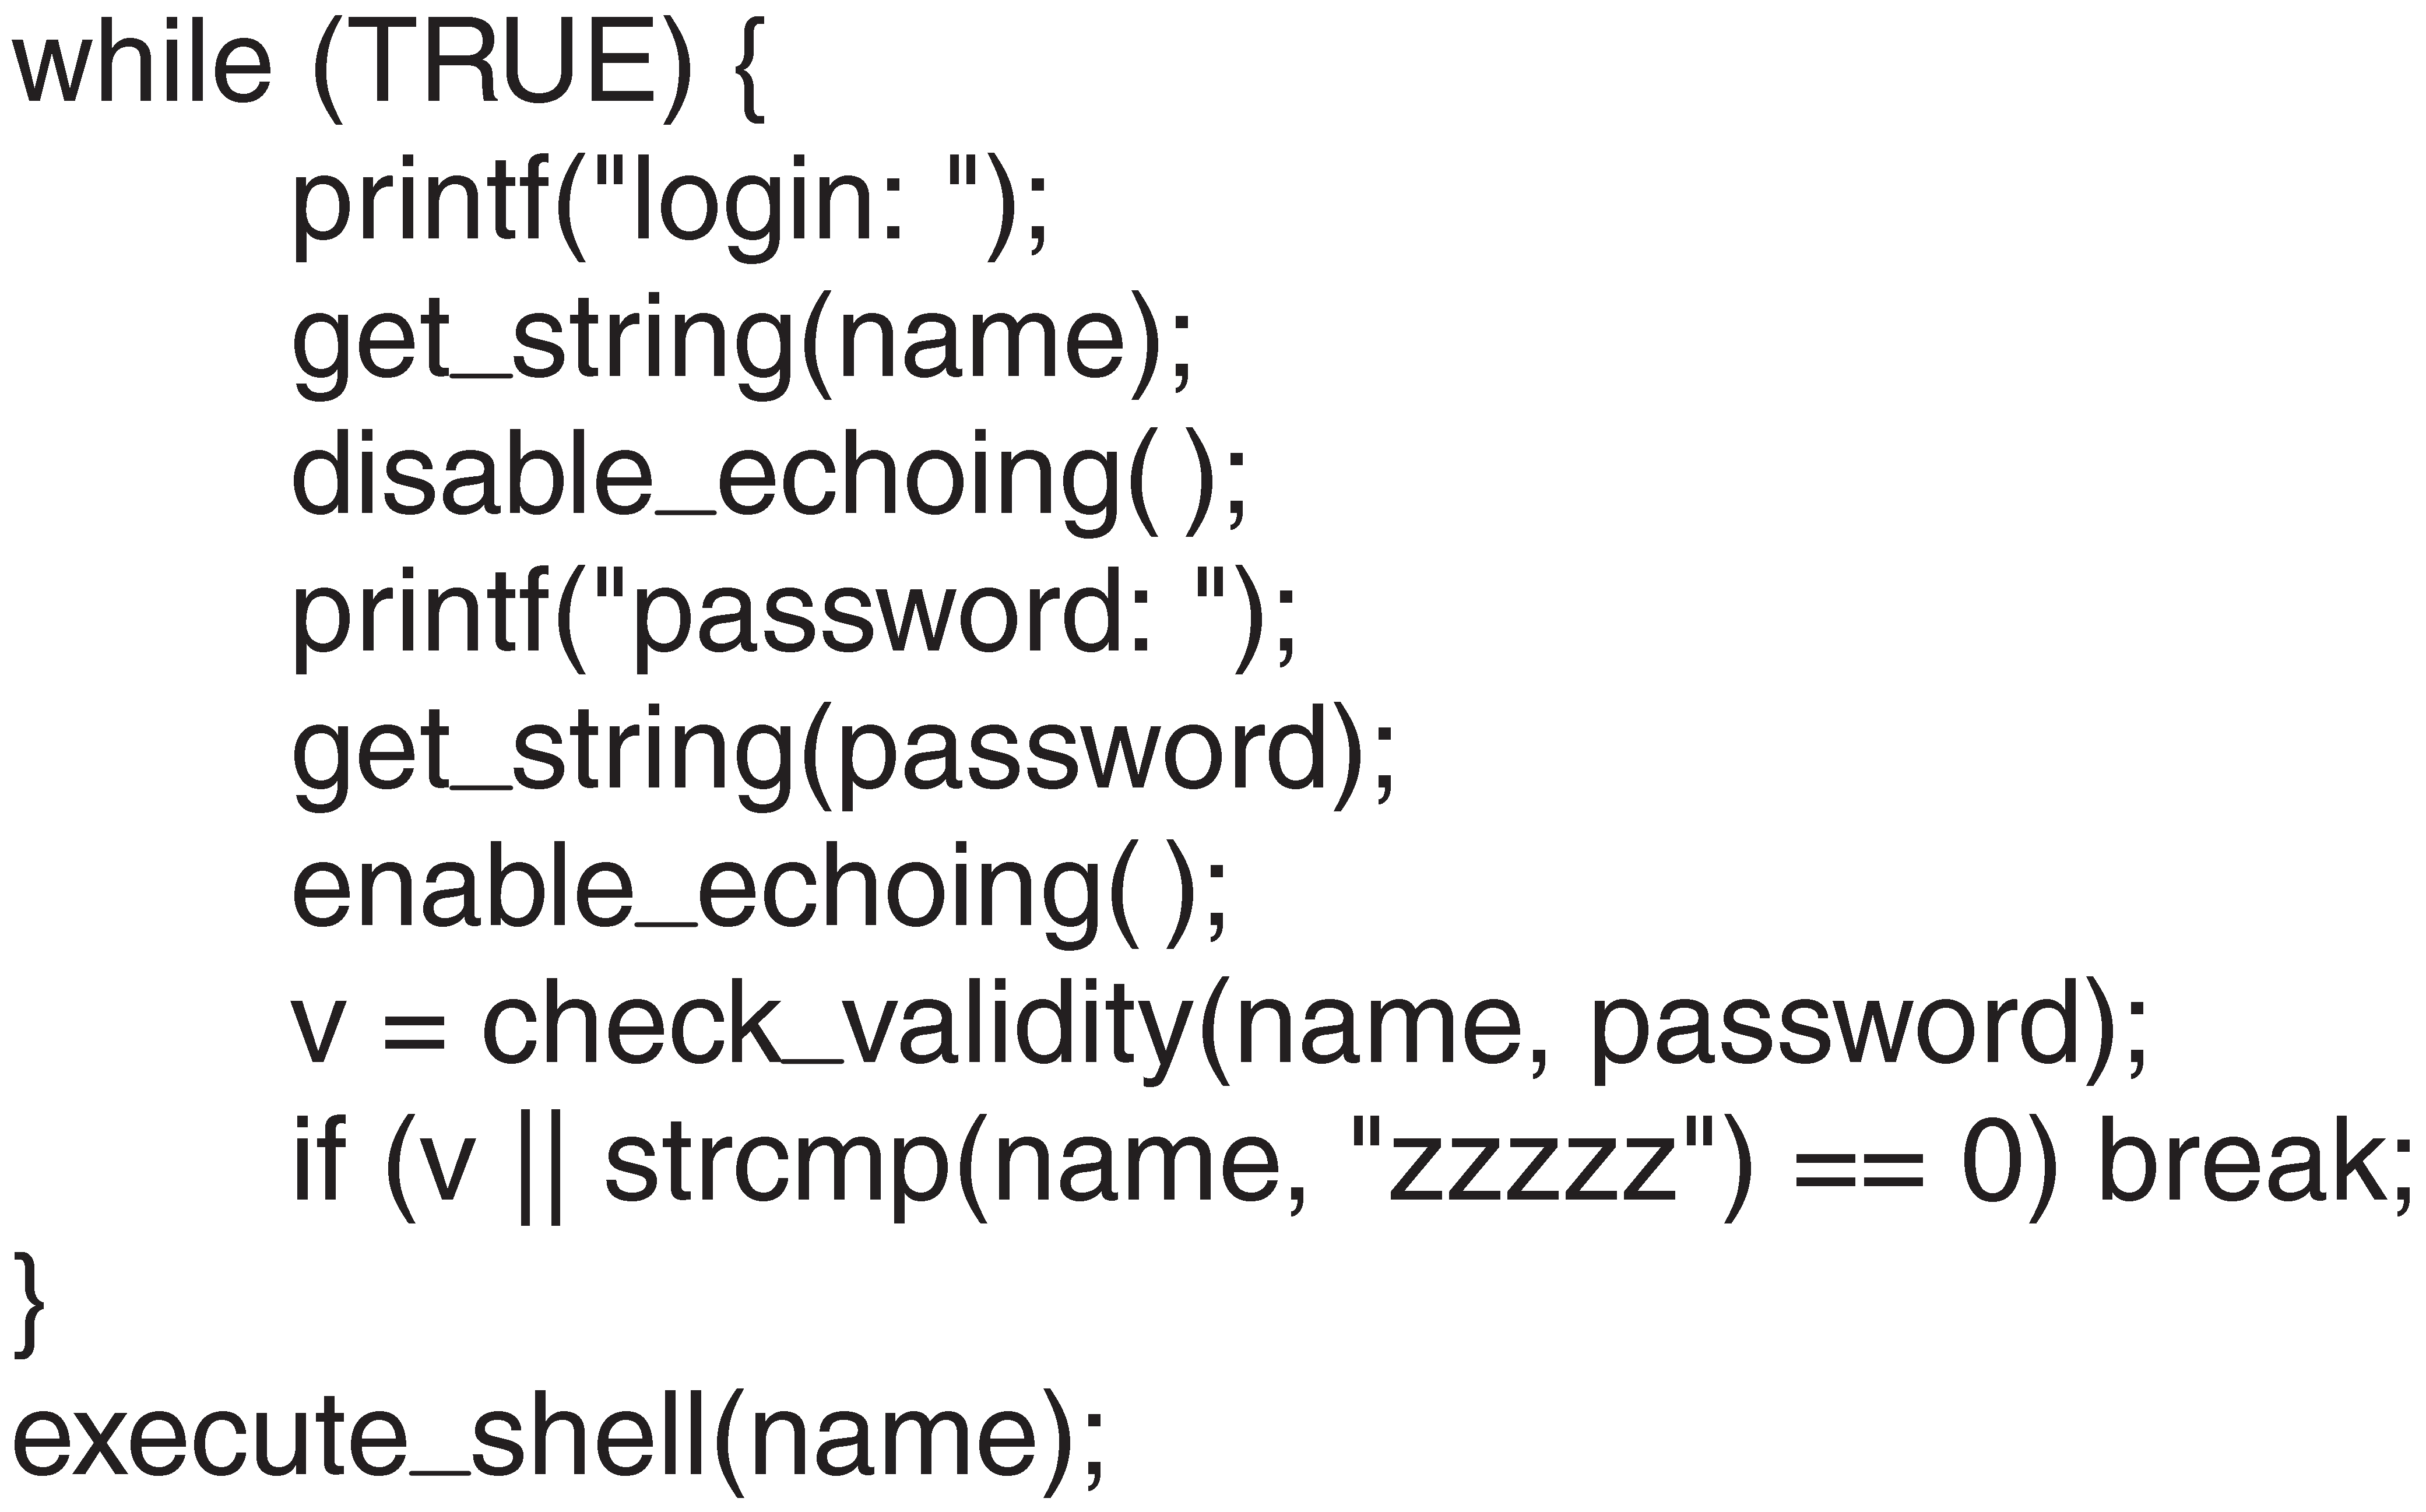
\includegraphics[width=0.55\textwidth]{back-door}
		\caption{A simple back door.}
	\end{figure}
	\end{frame}

	\begin{frame}
	\frametitle{Security Threats}
	\framesubtitle{Exploit Attacks -- Buffer Overflow}
	\begin{itemize}
	\setlength\itemsep{0.5em}
		\item No bound checks on arrays
		\item Intentionally overflow an array
		\item Insert malicious code in the array
	\end{itemize}
	%
	\begin{figure}
		\centering
		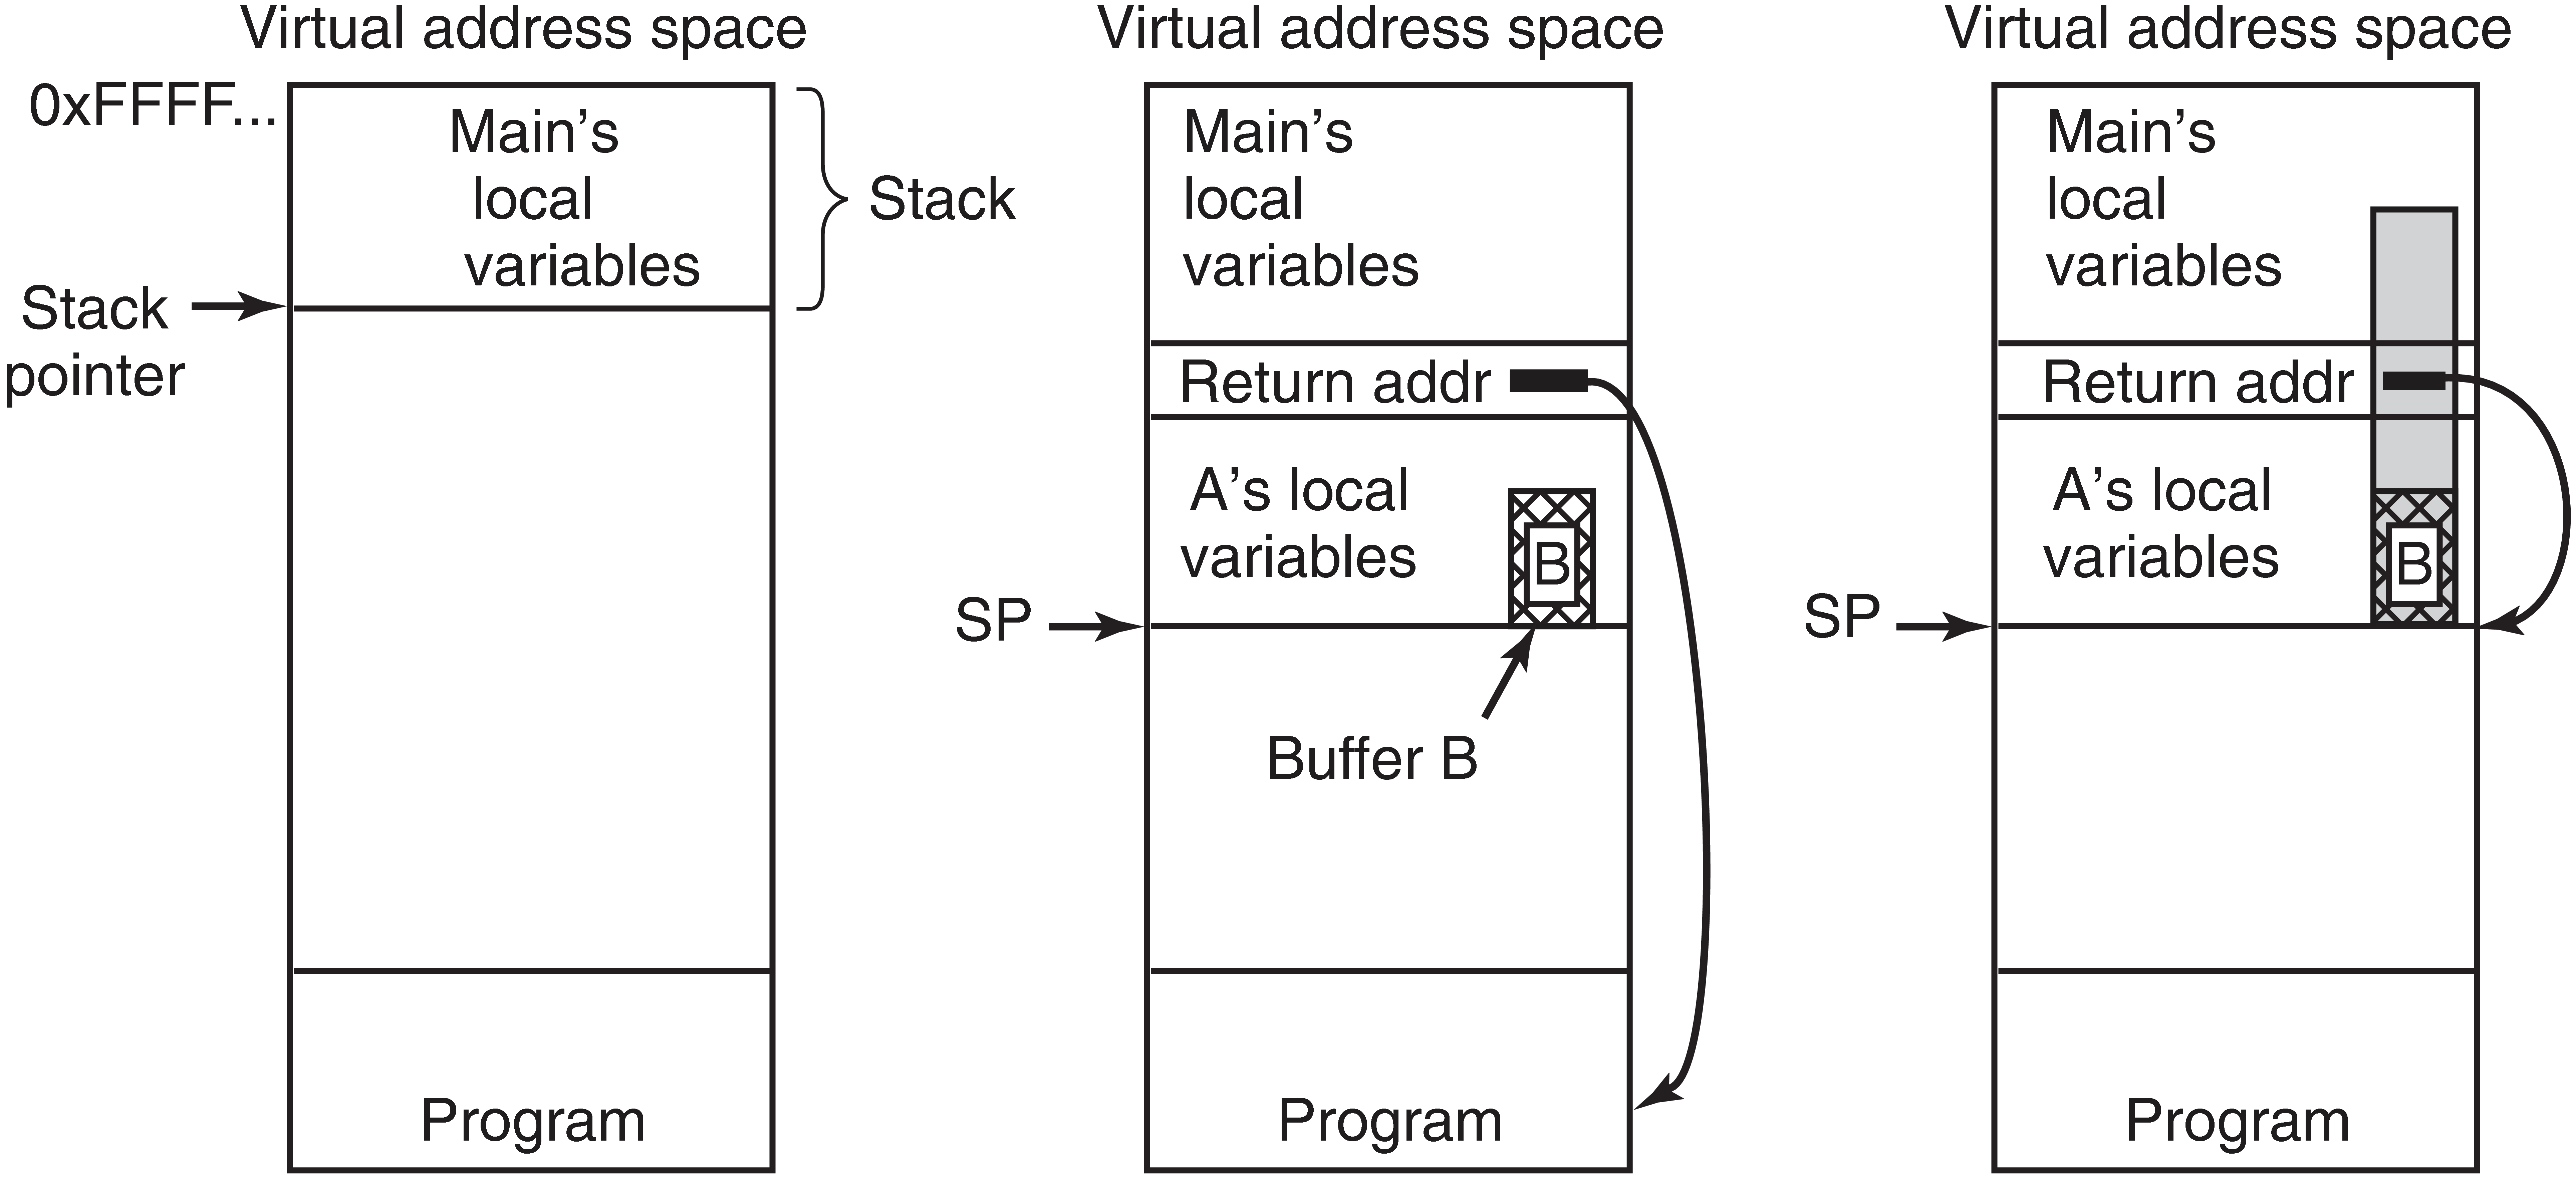
\includegraphics[width=0.75\textwidth]{buffer-overflow}
		\caption{Buffer overflow technique.}
	\end{figure}
	\end{frame}

	\begin{frame}
	\frametitle{Security Threats}
	\framesubtitle{Exploit Attacks -- Command Injection}
	\begin{itemize}
	\setlength\itemsep{0.5em}
		\item No validation on input fields
		\item External command runs the input field
		\item Inject malicious code in the input
	\end{itemize}
	%
	\begin{figure}
		\centering
		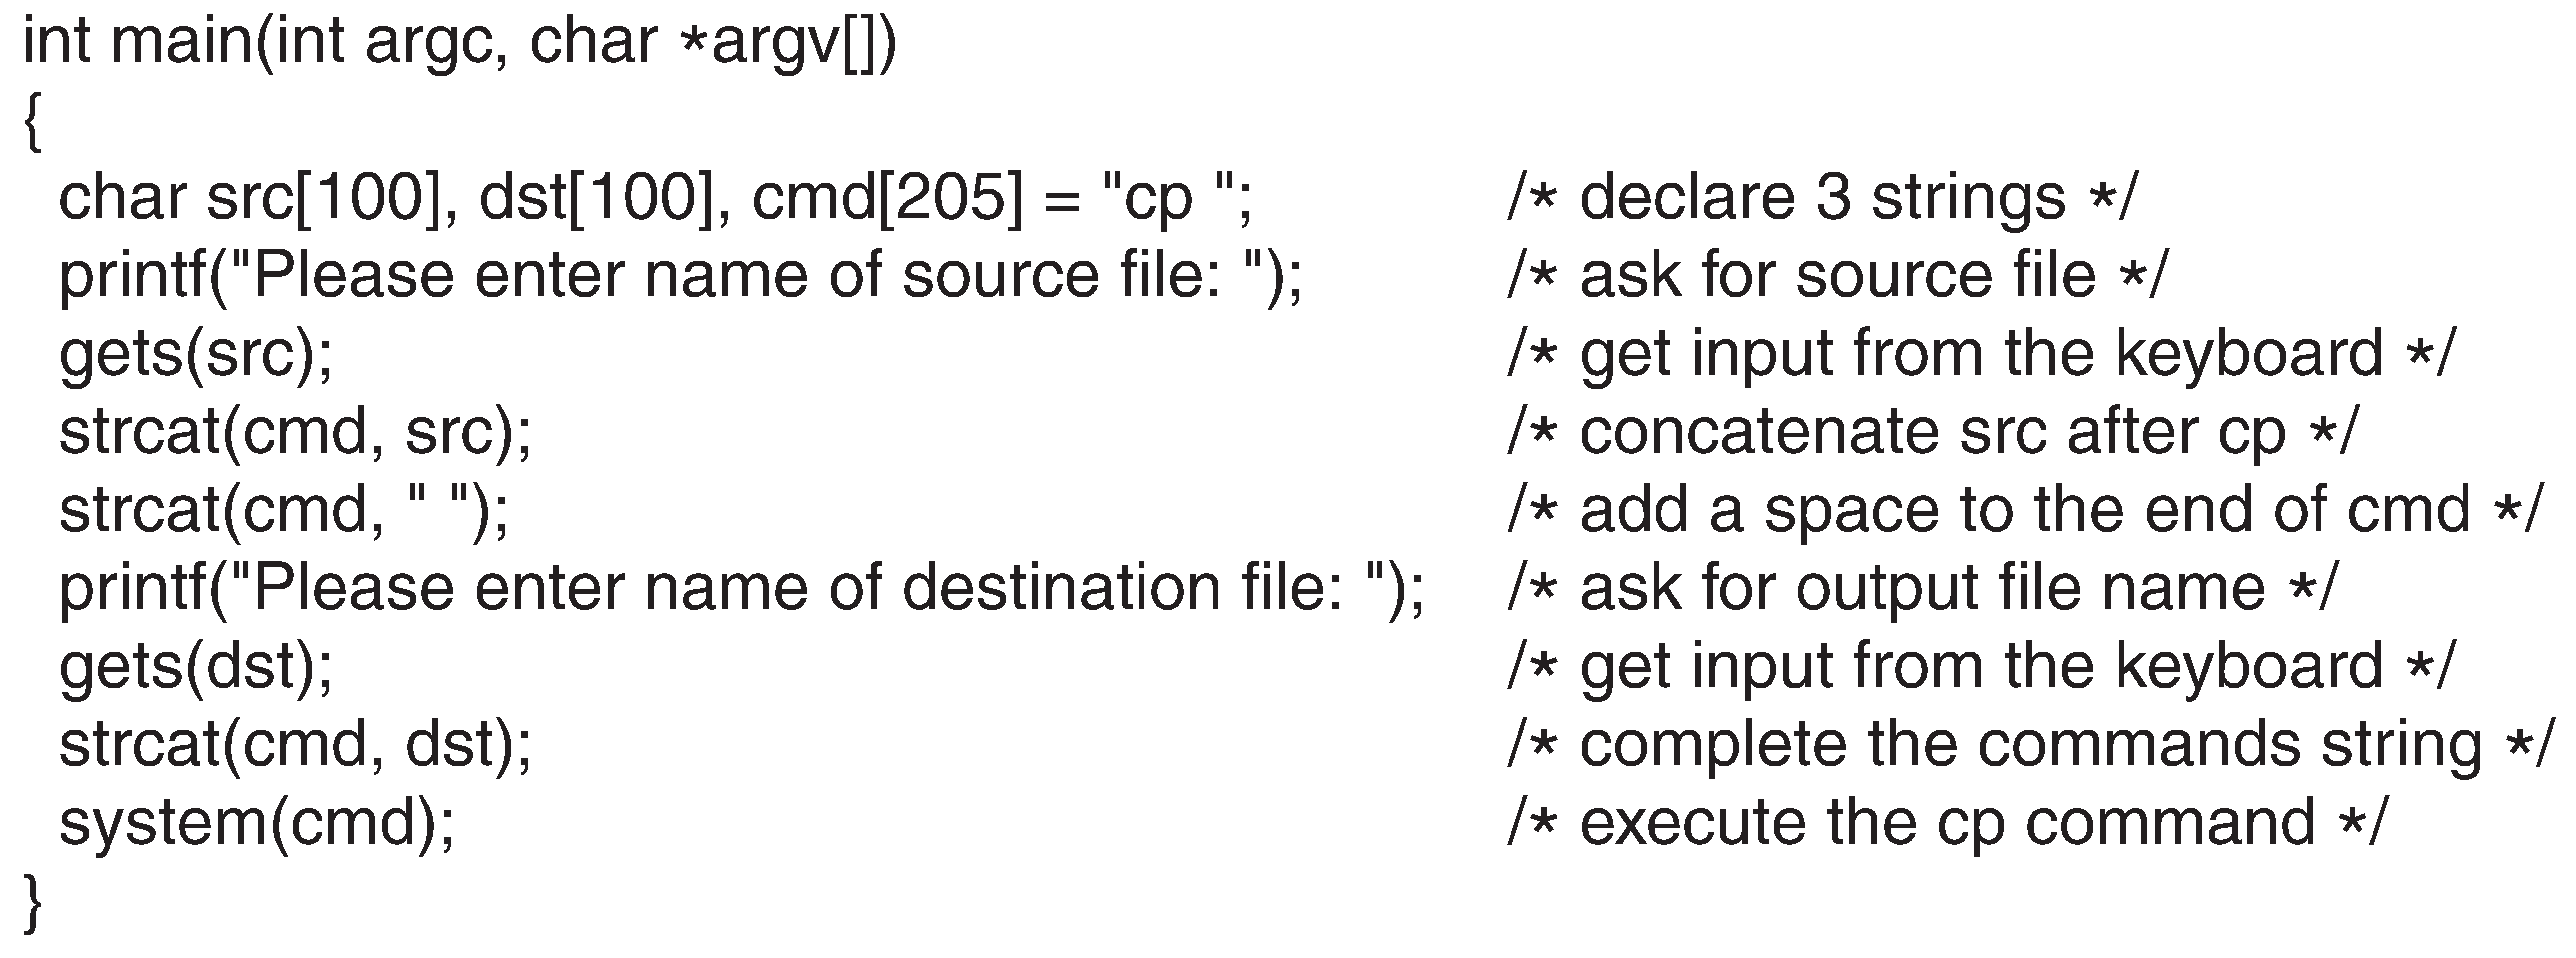
\includegraphics[width=0.80\textwidth]{command-injection}
		\caption{Command injection technique.}
	\end{figure}
	\end{frame}
	
	\begin{frame}
	\frametitle{Security Threats}
	\framesubtitle{Viruses}
	\begin{itemize}
	\setlength\itemsep{1.5em}
		\uncover<1->{
			\item Self-reproducing program
		}
		\uncover<2->{
			\item Payload with malicious code
			\begin{itemize}
				\item Spread chaos
				\item Monitor activity of users
				\item Take control over the remote machine
				\item Open a connection with a remote machine
			\end{itemize}
		}
		\uncover<3->{
			\item Several flavors
			\begin{itemize}
				\item Worms
				\item Trojan Horses
				\item Spywares
			\end{itemize}
		}
	\end{itemize}
	\end{frame}

	\begin{frame}
	\frametitle{Security Threats}
	\framesubtitle{Viruses}
	\begin{itemize}
	\setlength\itemsep{1.5em}
		\item Companion Virus
		\begin{itemize}
			\item Runs instead of a trusted program
		\end{itemize}

		\item Overwriting Virus
		\begin{itemize}
			\item Overwrites binary files with its code
		\end{itemize}

		\item Parasitic Virus
		\begin{itemize}
			\item Infects a binary file
		\end{itemize}

		\item Memory-Resident Virus
		\begin{itemize}
			\item Resides in-code either in user libraries or in the
			kernel
		\end{itemize}
	
		\item Boot Sector Virus
		\begin{itemize}
			\item Installs itself in the master boot record
		\end{itemize}
	\end{itemize}
	\end{frame}

	\begin{frame}
	\frametitle{Security Threats}
	\framesubtitle{Viruses -- Virus Types}
	\begin{itemize}
	\setlength\itemsep{1.0em}
		\item Head viruses
		\item Tail viruses
		\item Cavity viruses
	\end{itemize}
	%
	\begin{figure}
		\centering
		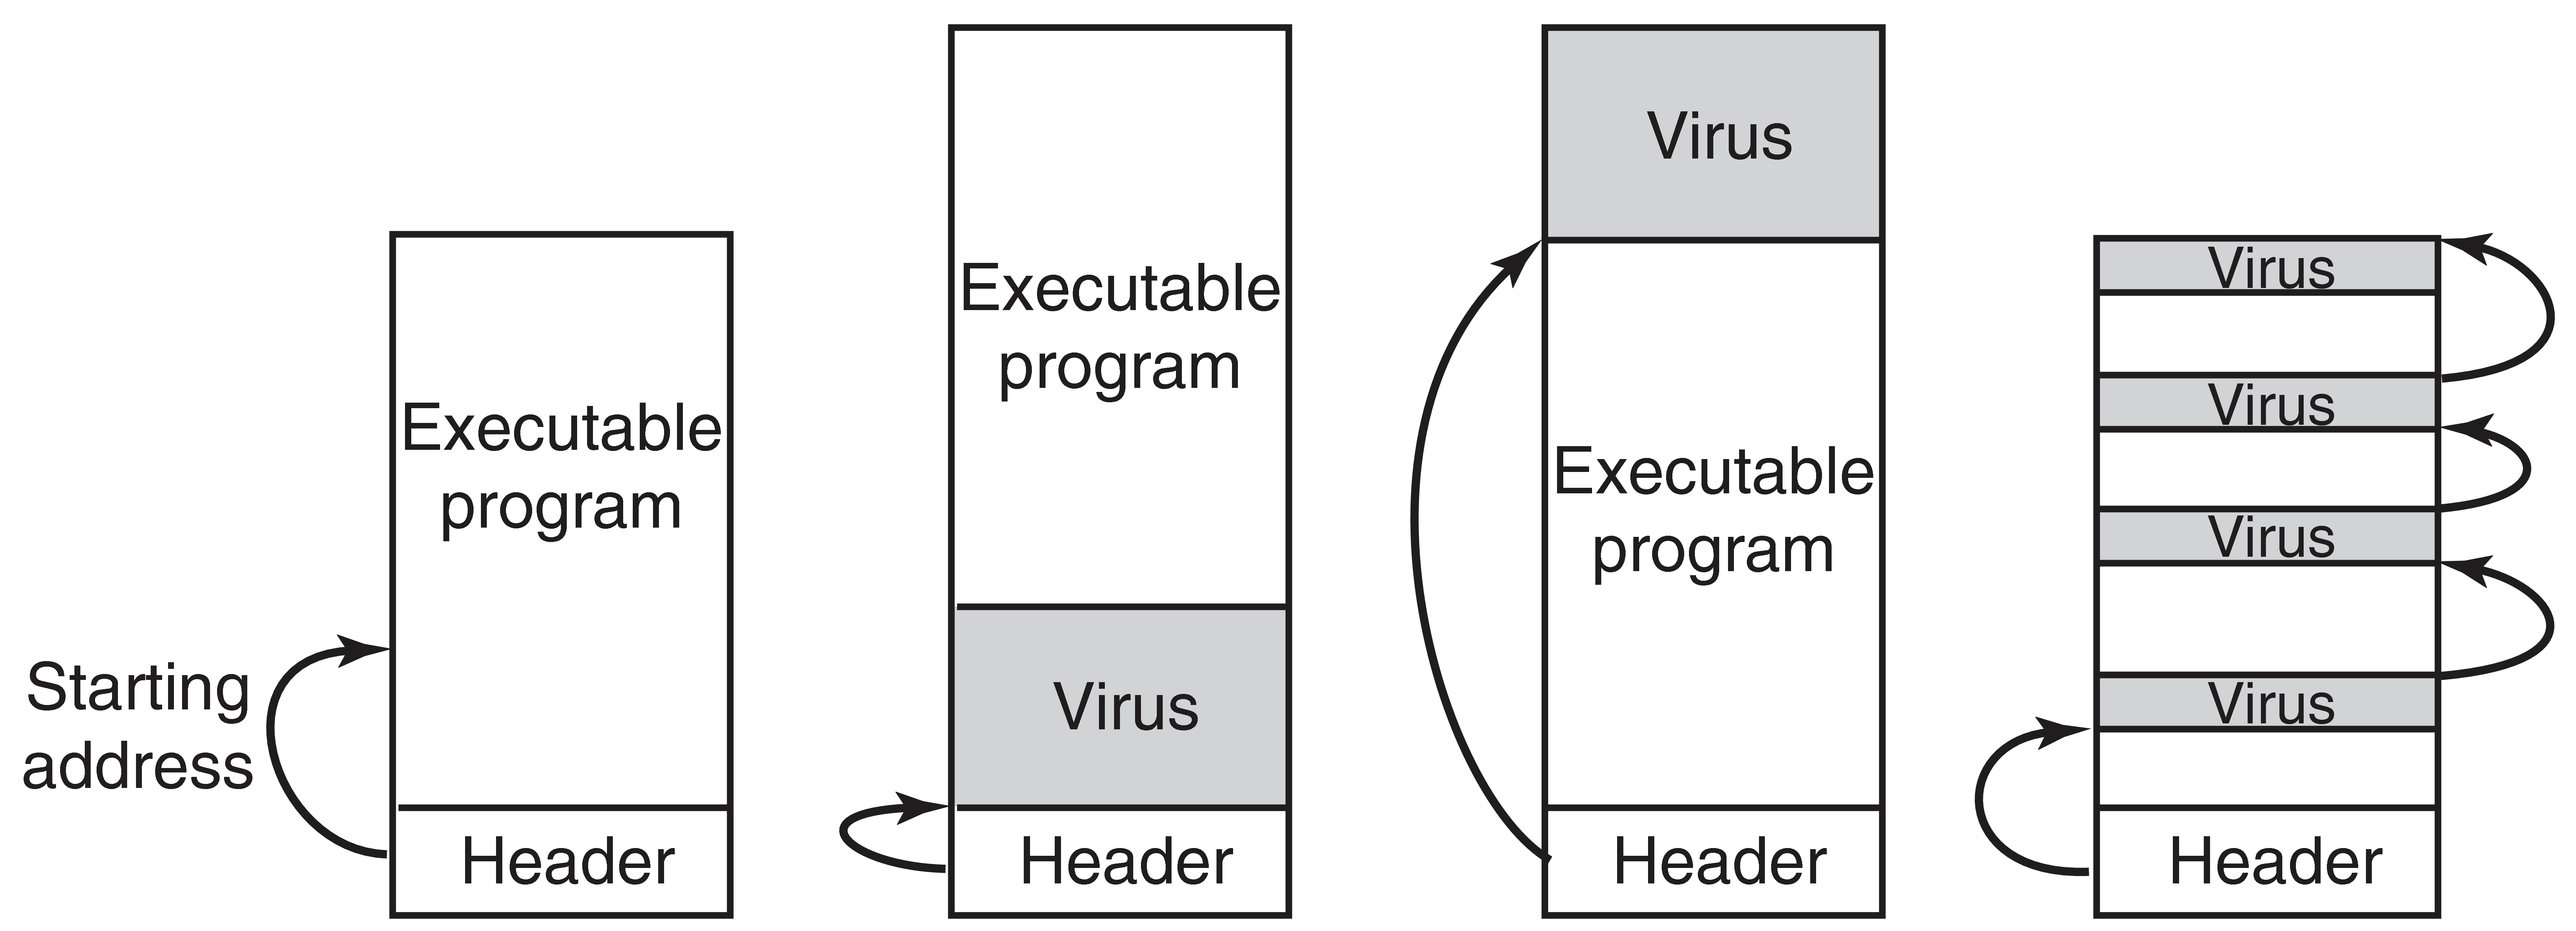
\includegraphics[width=0.8\textwidth]{virus-types}
		\caption{Parasitic virus types.}
	\end{figure}
	\end{frame}

	\begin{frame}
	\frametitle{Security Threats}
	\framesubtitle{Viruses -- Virus Compress and Encryption}
	\begin{itemize}
	\setlength\itemsep{1.0em}
		\item Compress: avoid file size check detection
		\item Encrypt: avoid signature detection
	\end{itemize}
	%
	\begin{figure}
		\centering
		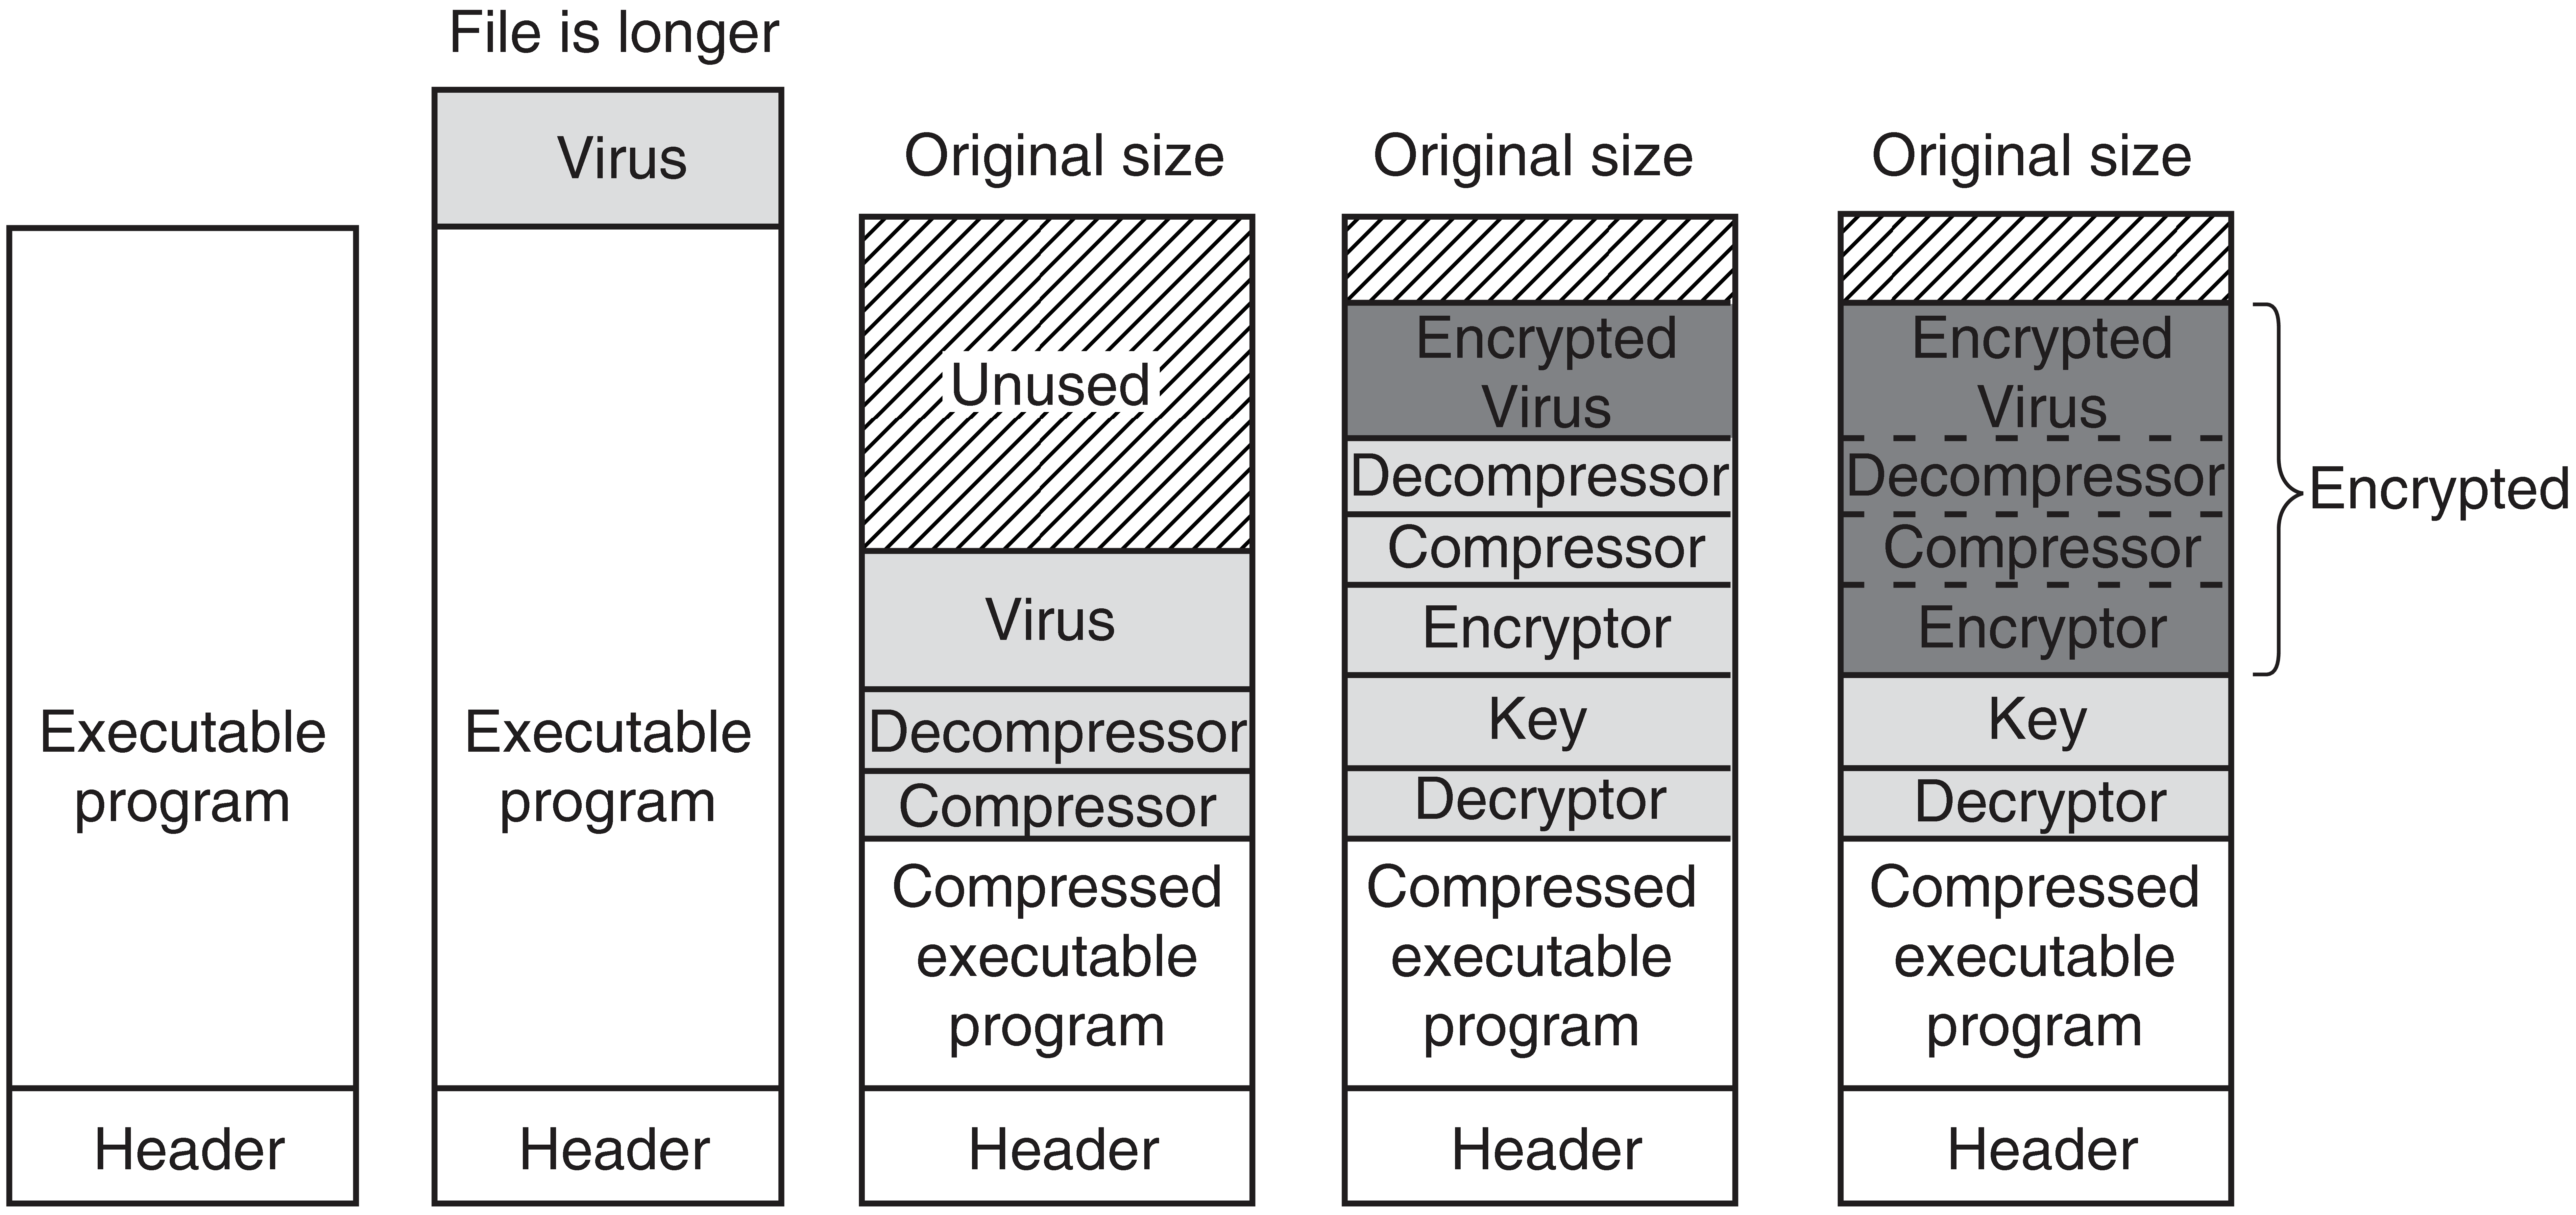
\includegraphics[width=0.8\textwidth]{virus-encryption}
		\caption{Virus encryption technique.}
	\end{figure}
	\end{frame}

	\begin{frame}
	\frametitle{Security Threats}
	\framesubtitle{Viruses -- Virus Mutation}
	\begin{itemize}
	\setlength\itemsep{1.0em}
		\item Avoid signature detection
	\end{itemize}
	%
	\begin{figure}
		\centering
		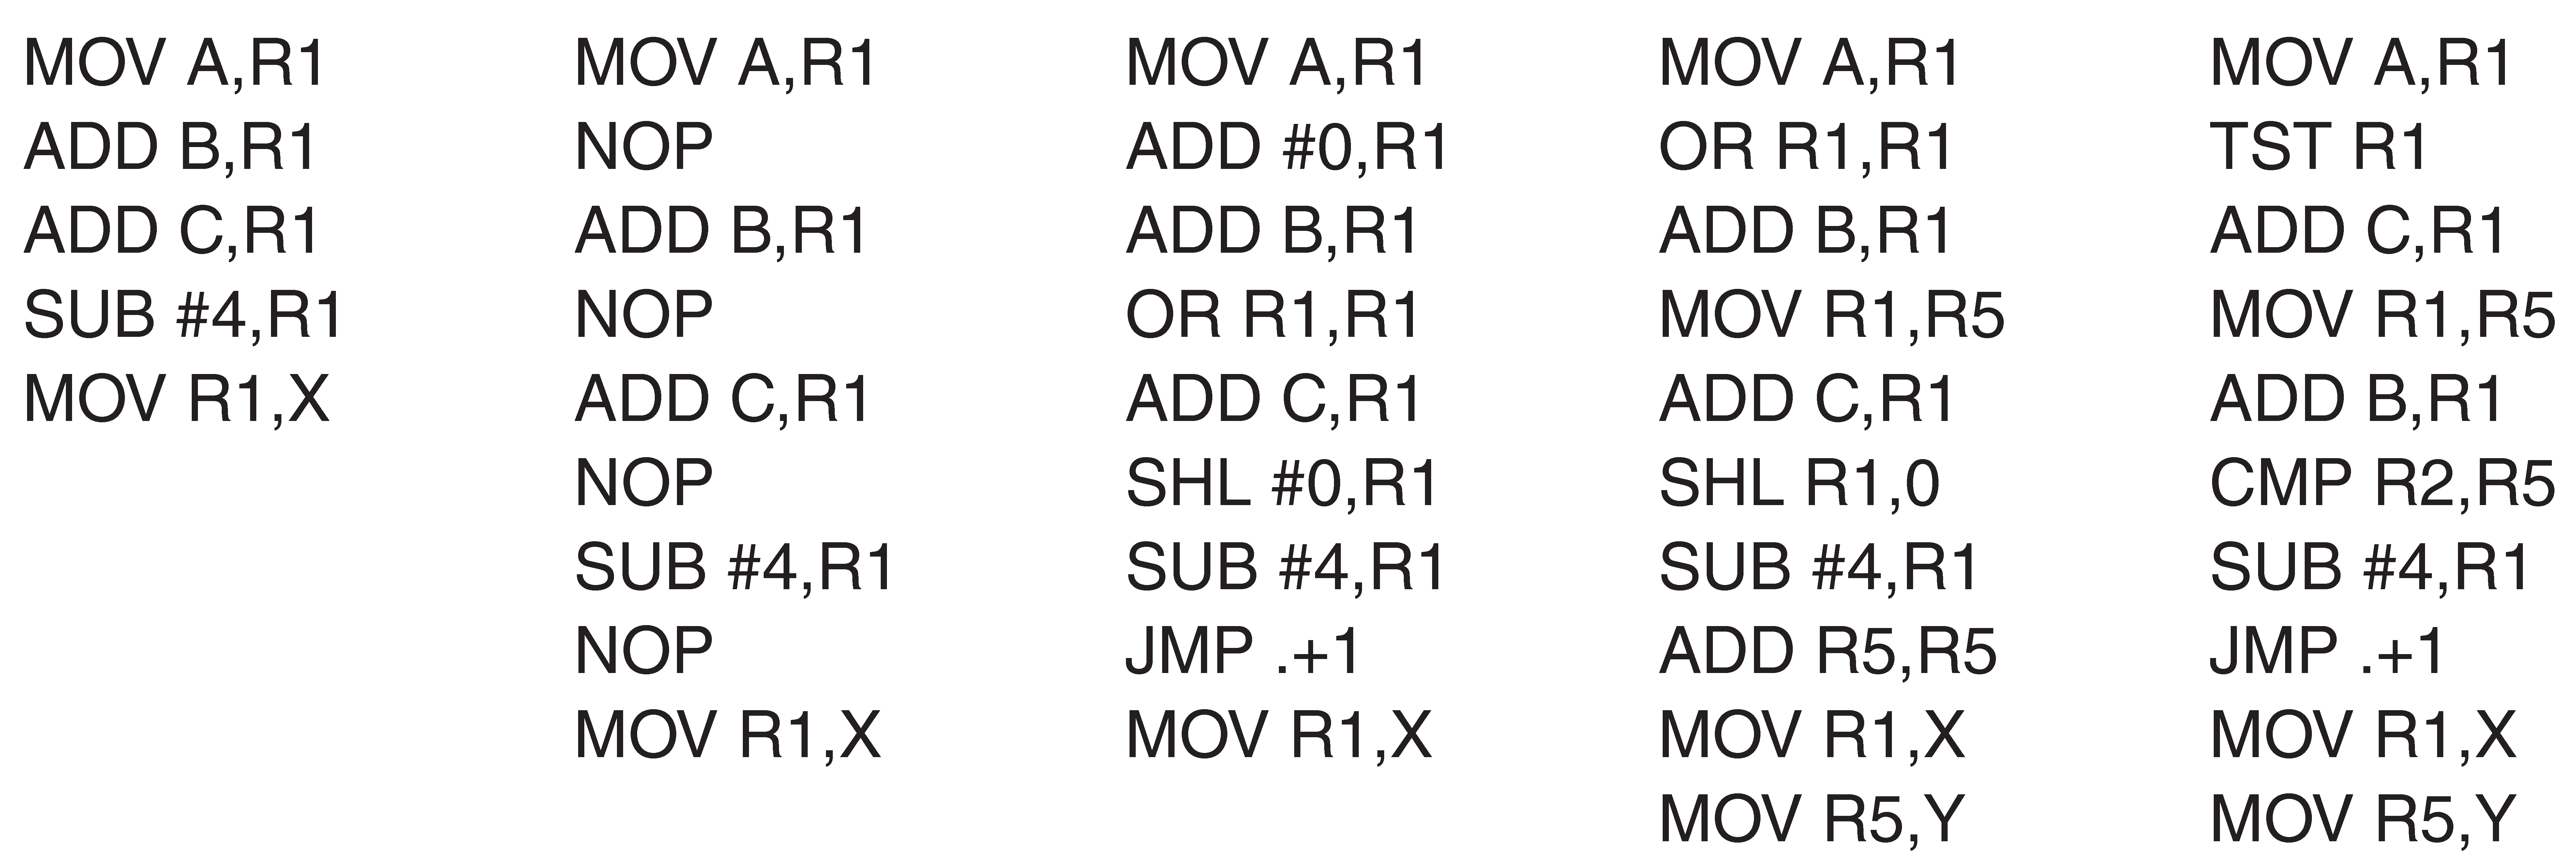
\includegraphics[width=0.8\textwidth]{virus-mutation}
		\caption{Virus mutation technique.}
	\end{figure}
	\end{frame}

\section{Defenses}

	\begin{frame}
	\frametitle{Defenses}
	\framesubtitle{Rules of Thumb}
	\begin{itemize}
	\setlength\itemsep{1.5em}
		\uncover<1->{
			\item Deny access by default
		}
		\uncover<2->{
			\item Always check for permissions
		}
		\uncover<3->{
			\item Give users minimum privileges
		}
		\uncover<4->{
			\item Authenticate users
		}
	\end{itemize}
	\end{frame}


	\begin{frame}
	\frametitle{Defenses}
	\framesubtitle{Cryptography}
	\begin{itemize}
	\setlength\itemsep{1.5em}
		\uncover<1->{
			\item Cornerstone technique that enables security
			\begin{itemize}
			\setlength\itemsep{0.5em}
				\item Data encryption
				\item Password scrambling
				\item Digital signatures
			\end{itemize}
		}
		\uncover<2->{
			\item Secrets should remain in secret
			\begin{itemize}
			\setlength\itemsep{0.5em}
				\item Encode a plaintext using a secret key
				\item Store/transmit encrypted data
				\item Decode encrypted data using a secret key
				\item Distribute encryption/decryption keys to trusted
				people
			\end{itemize}
		}
	\end{itemize}
	\end{frame}	

	\begin{frame}
	\frametitle{Defenses}
	\framesubtitle{Cryptography}
	\begin{figure}
		\centering
		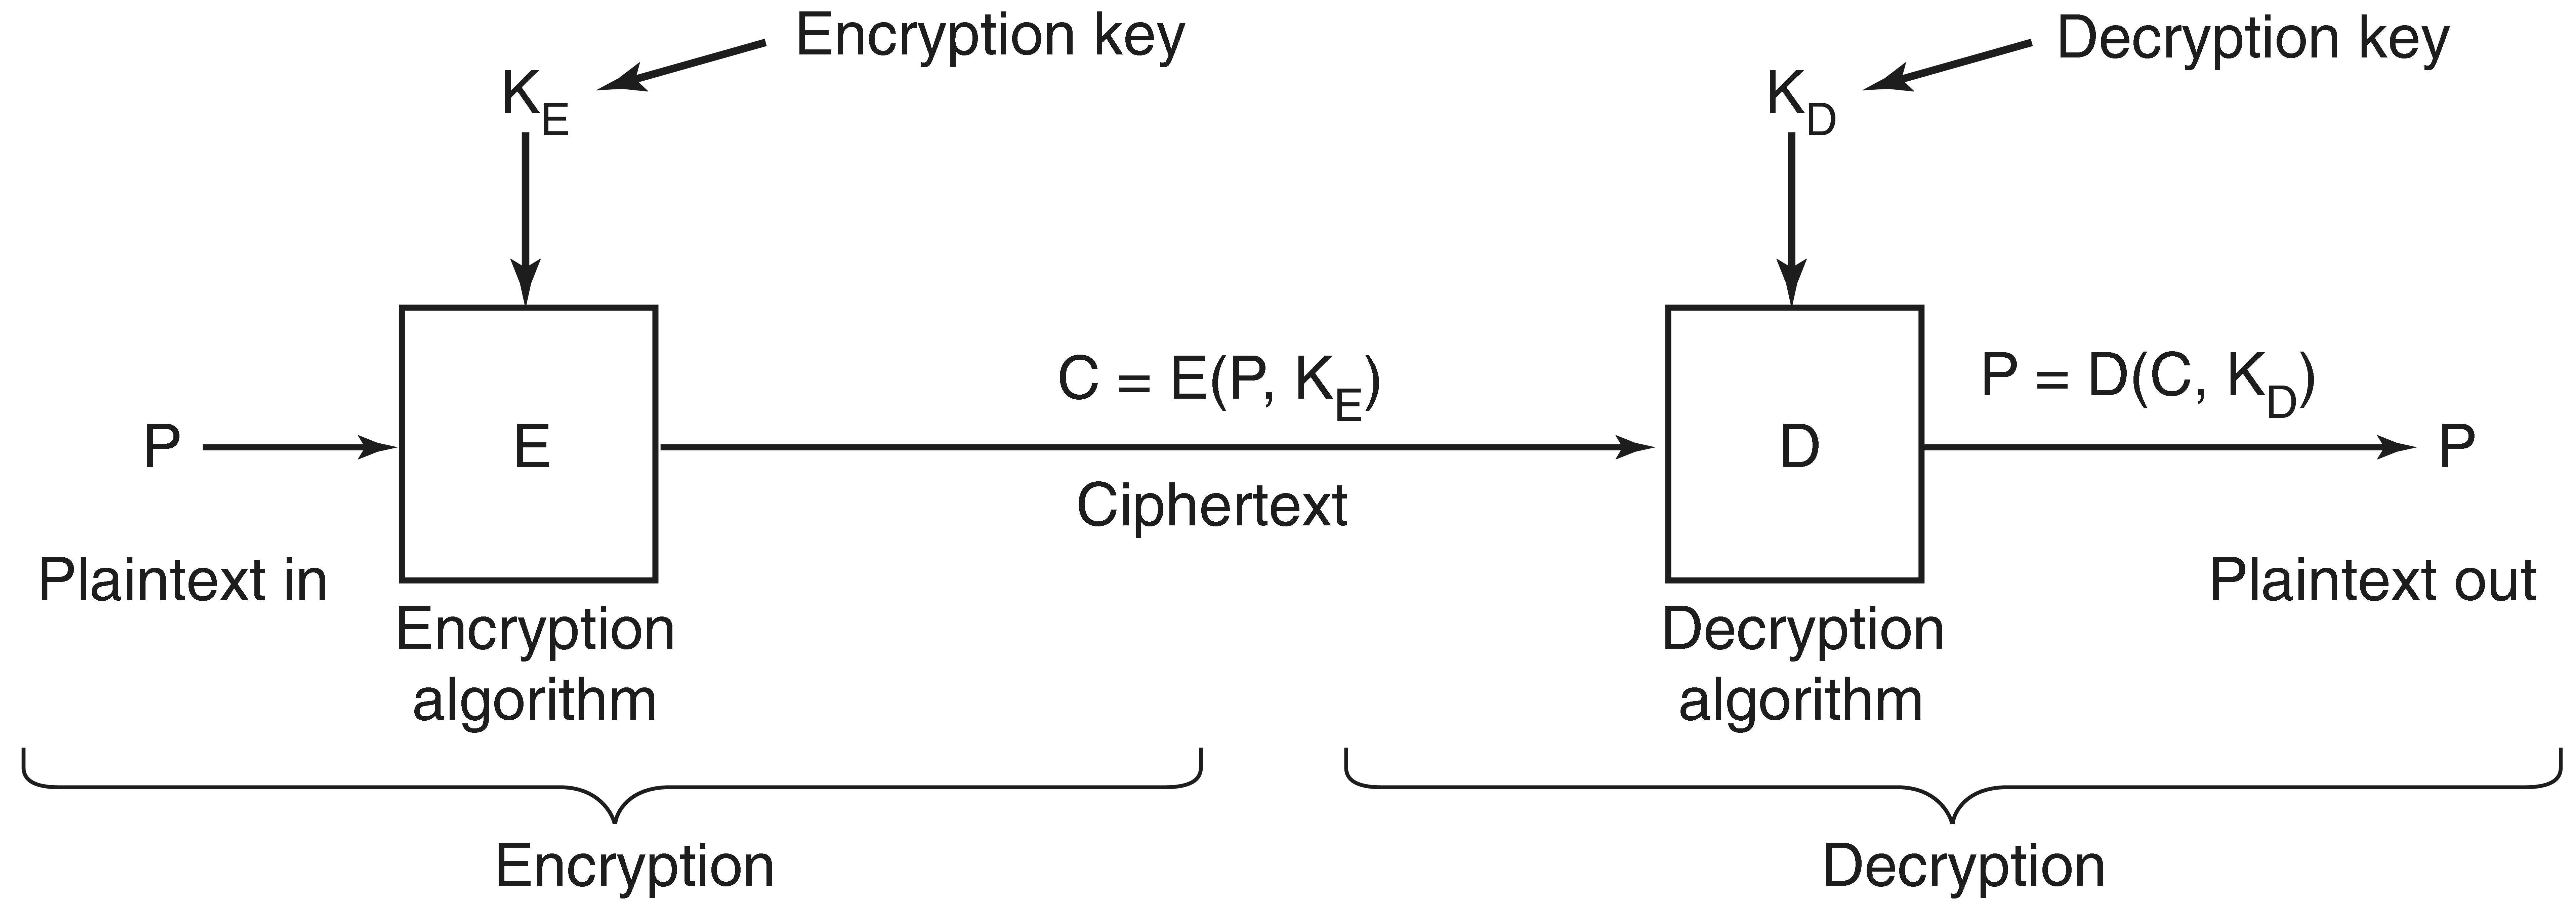
\includegraphics[width=1.00\textwidth]{cryptography}
		\caption{Cryptography in use.}
	\end{figure}
	\end{frame}	

	\begin{frame}
	\frametitle{Defenses}
	\framesubtitle{Cryptography}
	\begin{itemize}
	\setlength\itemsep{1.5em}
		\uncover<1->{
			\item Symmetric-Key Algorithms
			\begin{itemize}
			\setlength\itemsep{0.5em}
				\item Single key used for encryption/decryption
				\item Key should kept in secret
				\item Caesar Encryption
				\item Data Encryption Standard (DES)
				\item Advanced Encryption Standard (AES)
			\end{itemize}
		}
		\uncover<2->{
			\item Asymmetric-Key Algorithms
			\begin{itemize}
			\setlength\itemsep{0.5em}
				\item Public key used for encryption
				\item Private key for decryption
				\item  Diffie–Hellman Key Exhange Protocol
				\item ElGamal Encryption
				\item Rivest-Shamir-Adleman Encryption (RSA)
			\end{itemize}
		}
	\end{itemize}
	\end{frame}

	\begin{frame}[t]
	\frametitle{Defenses}
	\framesubtitle{Firewalls}
	\begin{itemize}
	\setlength\itemsep{1.0em}
		\uncover<1->{
			\item Problems on network connectivity
			\begin{itemize}
			\setlength\itemsep{0.5em}
				\item Traffic sniffing
				\item External invasions
			\end{itemize}
		}
		\uncover<2->{
			\item Firewalls
			\begin{itemize}
			\setlength\itemsep{0.5em}
				\item Keep intruders out
				\item Ensure data integrity on in/out traffic
				\item Set of rules state what is allowed
			\end{itemize}
		}
	\end{itemize}
	%
	\only<2>{
		\begin{figure}
			\centering
			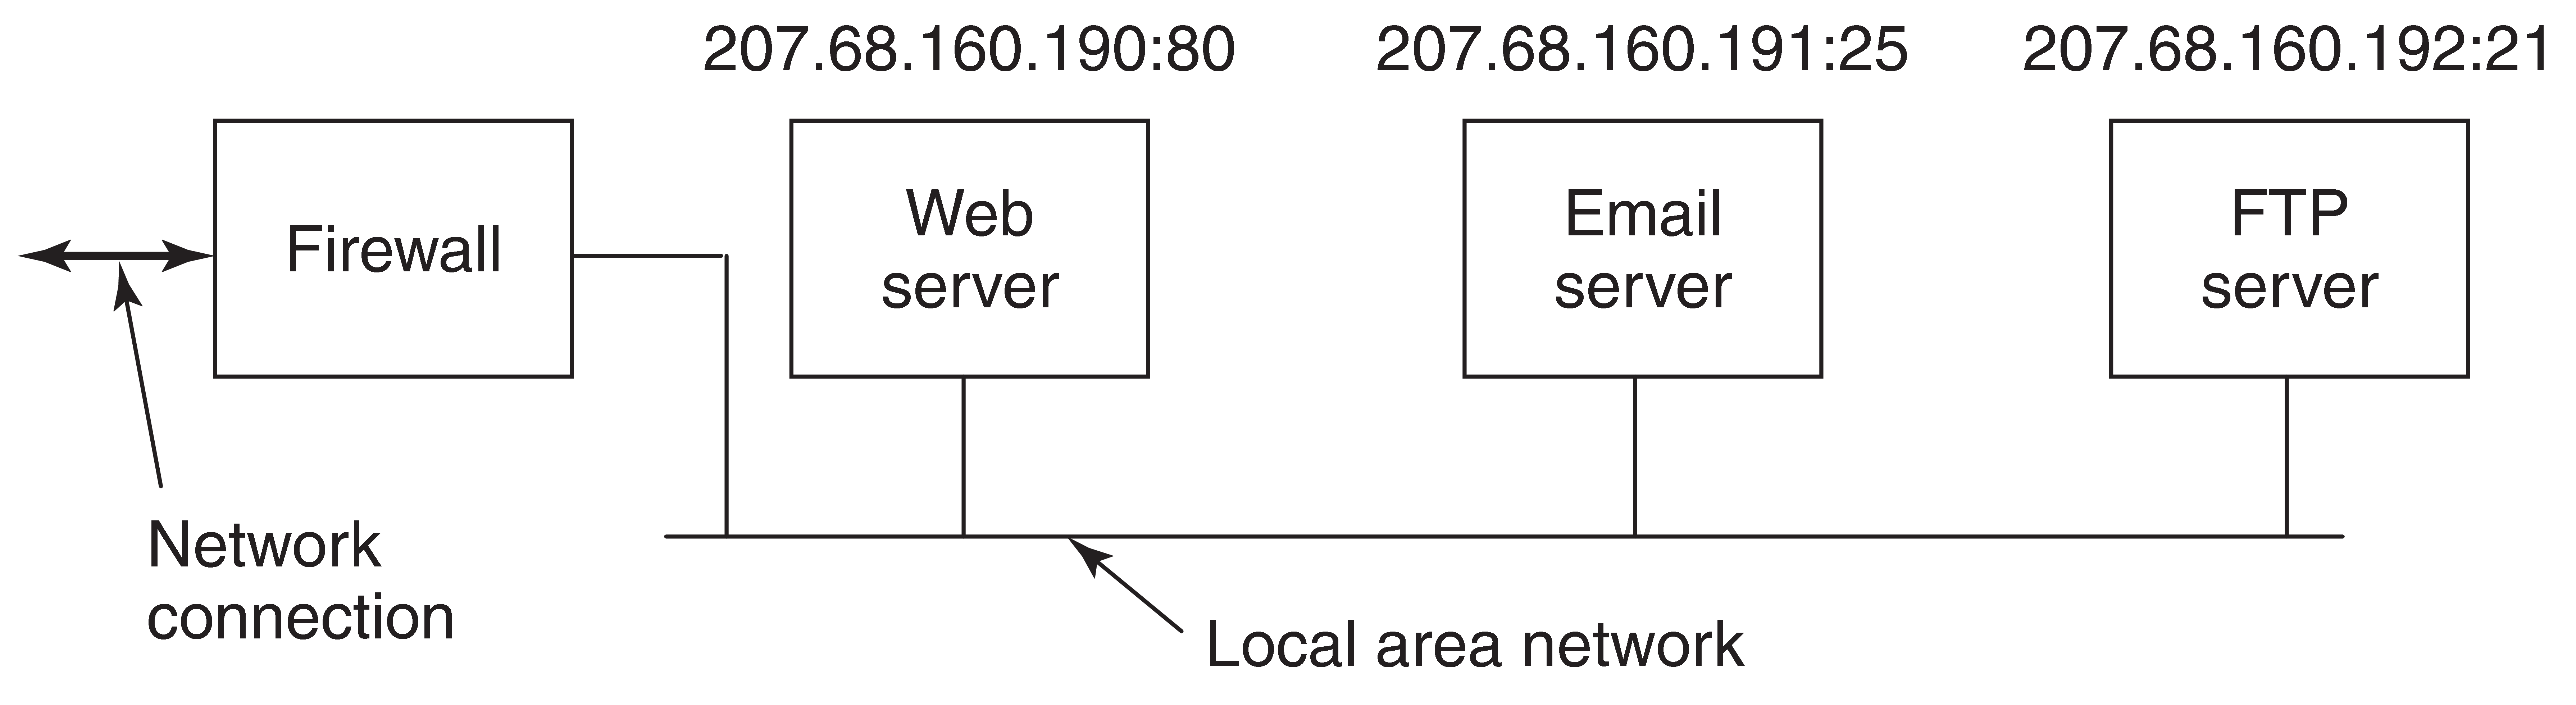
\includegraphics[width=0.70\textwidth]{hardware-firewall}
			\caption{Hardware firewall.}
		\end{figure}
	}
	\end{frame}

	\begin{frame}
	\frametitle{Defenses}
	\framesubtitle{Firewalls}
	\begin{itemize}
	\setlength\itemsep{1.0em}
		\uncover<1->{
			\item Hardware firewalls
			\begin{itemize}
			\setlength\itemsep{0.5em}
				\item Protect machines in a LAN
				\item Dedicated device placed between the ISP and
				LAN
			\end{itemize}
		}
		\uncover<2->{
			\item Software firewalls
			\begin{itemize}
			\setlength\itemsep{0.5em}
				\item Protect a single machine
				\item Dedicated software in the operating system
			\end{itemize}
		
		}
		\uncover<3->{
			\item Stateless firewalls
			\begin{itemize}
			\setlength\itemsep{0.5em}
				\item Inspect the header of every network package
			\end{itemize}
		}
		\uncover<4->{
			\item Stateful firewalls
			\begin{itemize}
			\setlength\itemsep{0.5em}
				\item Keeps track of connections
			\end{itemize}
		}
		\uncover<5->{
			\item Intrusion detect system
			\begin{itemize}
			\setlength\itemsep{0.5em}
				\item Inspects the content of network packages
			\end{itemize}
		}
	\end{itemize}
	\end{frame}

	\begin{frame}
	\frametitle{Defenses}
	\framesubtitle{Antivirus}
	\begin{itemize}
	\setlength\itemsep{1.5em}
		\uncover<1->{
			\item Malicious software
			\begin{itemize}
			\setlength\itemsep{0.5em}
				\item Information stealing
				\item System crash
			\end{itemize}
		}
		\uncover<2->
		{
			\item Fighting heuristics (antivirus)
			\begin{itemize}
			\setlength\itemsep{0.5em}
				\item Virus scanners
				\item Integrity checkers
				\item Behavioral checkers
			\end{itemize}
		}
	\end{itemize}
	\end{frame}

	\begin{frame}
	\frametitle{Defenses}
	\framesubtitle{Antivirus -- Virus Scanners}
	\begin{itemize}
	\setlength\itemsep{1.5em}
		\uncover<1->{
			\item Infect goat files (dummy programs)
		}
		\uncover<2->{
			\item Isolate the virus signature (virus code)
		}
		\uncover<3->{
			\item Enter the virus code in a data base
		}
		\uncover<4->{
			\item Scan executable files seeking for virus signatures
			\begin{itemize}
				\item Heuristic search
			\end{itemize}
		}
	\end{itemize}
	\end{frame}
	
	\begin{frame}
	\frametitle{Defenses}
	\framesubtitle{Antivirus -- Integrity Checkers}
	\begin{itemize}
	\setlength\itemsep{1.5em}
		\uncover<1->{
			\item Scan the disk from viruses (virus scan)
		}
		\uncover<2->{
			\item Compute checksum for executable files
			\begin{itemize}
				\item Hash functions: SHA-1, SHA-2 and MD5
			\end{itemize}
		}
		\uncover<3->{
			\item Store the checksum somewhere safe
		}
		\uncover<4->{
			\item On next scan do checksumming
			\begin{itemize}
				\item Infected files will have unmatching checksums
			\end{itemize}
		}
	\end{itemize}
	\end{frame}

	\begin{frame}
	\frametitle{Defenses}
	\framesubtitle{Antivirus -- Behavioral Checkers}
	\begin{itemize}
	\setlength\itemsep{1.5em}
		\uncover<1->{
			\item Antivirus resides in memory
		}
		\uncover<2->{
			\item Wrap system calls
		}
		\uncover<3->{
			\item Monitor all the activity in the system
		}
		\uncover<4->{
			\item Deny suspicious actions
		}
	\end{itemize}
	\end{frame}

	\begin{frame}
	\frametitle{Defenses}
	\framesubtitle{Authentication}
	\begin{itemize}
	\setlength\itemsep{1.5em}
		\uncover<1->{
			\item Fake users
			\begin{itemize}
				\item Malicious actions
			\end{itemize}
		}
		\uncover<2->{
			\item Authenticate users on login
			\begin{itemize}
				\item Login name
				\item Password
			\end{itemize}
		}
		\uncover<3->{
			\item Store credentials somewhere safe
			\begin{itemize}
				\item File with restricted access permissions
				\item Encrypted file
			\end{itemize}
		}
		\uncover<4->{
			\item Biometry authentication 
			\begin{itemize}
				\item Fingerprinting
				\item Iris recognition
				\item DNA profiling
			\end{itemize}
		}
	\end{itemize}
	\end{frame}

\end{document}
